\documentclass[]{article}

\usepackage[left=0.5in, right=0.5in, top=0.5in]{geometry}
\usepackage{hyperref}
\usepackage{graphicx}

\setlength\parindent{0pt}

\hypersetup{
	colorlinks=true,
	linkcolor=blue,
	filecolor=blue,      
	urlcolor=blue
}

%opening
\title{Automated Plant Care}
%\author{Justin Herter} 
\date{}

\begin{document}

\maketitle


\section{Introduction}
The goal of this project is to implement reliable automation for plant care.  Taking care of plants that yield something of value to the caretaker or his or her employer boils down to supplying the proper levels of light, hydration, and nutrients.  Of these, the first two typically require the caretaker's attention at least once per day.  The most severe potential consequence of neglect is, of course, death of the plant, which renders the entire effort futile.
\\\\
The situation at hand involves a chronically negligent plant caretaker coupled with a low-light environment due to a large bush obstructing the only window.  What is documented here are the steps involved to establish a back-end for the automation itself that is paired with an informative front-end that also sends alerts for key events, e.g. a malfunctioning pump.

\section{System Overview}
The two fundamental pieces of equipment are the light and the pump, and what they both have in common is that they run on AC power.  Obviously, the controller for all of this -- a Raspberry Pi -- is only equipped to handle DC circuits at either 3.3 or 5 volts.  While it's possible to do something with relays, nobody wants to explain their neat project to an angry fire marshal.  Thus, for safety reasons, it has been elected to use a radio frequency (RF) transmitter paired with RF outlet switches to enable switching of the pump and light.  This has an added benefit of greater freedom for routing power.  The remainder of equipment to be used is given in the table below, and Fig. \ref{fig:schematic} provides a schematic.

\begin{table}[h]
\centering
\caption{Equipment specifications for plant care and monitoring.}
\begin{tabular}{l|l|r }
\textbf{Item} & \textbf{Purpose} & \textbf{Seller or Spec} \\ \hline
AC outlet switches & Allow RF control of AC appliances & \href{https://www.amazon.com/gp/product/B00DQELHBS/ref=ppx_yo_dt_b_search_asin_title?ie=UTF8\&psc=1}{Amazon} \\ \hline
Hygrometer & Monitoring of soil moisture & \href{https://www.aliexpress.com/item/32700826684.html?spm=a2g0s.9042311.0.0.770c4c4dQ7v1Z2}{AliExpress} \\ \hline 
Pump & Supply water to plant & \href{https://www.amazon.com/gp/product/B00EWENMAU/ref=ppx_yo_dt_b_search_asin_title?ie=UTF8&psc=1}{Amazon} \\ \hline 
Light & Provide correct spectrum for plant & Erligpowht 45 W grow light \\ \hline
Photoresistor & Ensure light is operating & GM5539 \\ \hline
Raspberry Pi & Runs at least the back-end & Raspberry Pi 3B \\ \hline
Raspberry Pi camera & Visual of plant and maybe time-lapse & V2 \\ \hline
Teensy 3.2 & Report analog sensor data & \href{https://www.amazon.com/gp/product/B015QUPO5Y/ref=ppx_yo_dt_b_search_asin_title?ie=UTF8&psc=1}{Amazon} 
\end{tabular}
\end{table}

\subsection{Operation}
The most trivial part of how the system will operate pertains to the light, which will run on a 12 hour on/off schedule.  Half-way through the day portion, the Raspberry Pi will take a still image of the plant.  The photoresistor will be used to ensure the light is working as it should.
\\\\
Next up is the pump operation.  When the hygrometer indicates dry soil, the pump will operate for a brief TBD interval.  This pump will be submerged in a reserve of water that will have a simple circuit that's nominally closed by the water itself until the reserve is nearing depletion.


\newpage
\subsection{Front-End Requirements}
The front-end will provide a simple, vertically scrolling interface with metrics about delivery of light and water to the plant in the form of two time-series plots for the last 24 hours.  Vertical axes will be the light level from the photoresistor and the moisture level from the hygrometer, respectively.
\\\\
Below the plots, there will be status indicators for the light level, moisture level, and water reserve level.  These will be boolean in nature, and the plant care-taker shall be notified in some way when one of these strays from nominal.  At the bottom of the interface, the most recent picture of the plant will be displayed.
\\\\
Hosting of the front-end will be on an AWS instance running an AMI generated by Packer and provisioned via Terraform.  On this instance, a web server and a database will run in Docker containers orchestrated by Docker Compose.  The web page will be open to the web, and everything else will only be open to the public IP of where the Pi is located.

\section{Sensors and Circuits}
\subsection{RF Outlets}
The starting point is to establish RF capability between the Pi and the RF outlets, which was accomplished by following the steps put forth by GitHub user timeland's \href{https://timleland.com/wireless-power-outlets/}{blog post} and the associated repository \href{https://github.com/timleland/rfoutlet}{rfoutlet}.  The basic procedure is to use an RF receiver to decode signals from the remote that came with the outlets, then use the RF transmitter to emulate the signal for a given channel.  This yielded the codes given in the table below, and Fig. \ref{fig:rf_circuit} shows the setup used.  Also, since it's not explicitly called out, the transmitter and receiver use wiring pi pins zero and two, respectively.  


\begin{table}[h]
\centering
\caption{Codes transmitted by RF outlet remote.}
\begin{tabular}{l|r|r}
	\textbf{Channel} & \textbf{On} &	\textbf{Off}
\\ \hline
	1 &	1398067	& 1398076
\\ \hline
	2 &	1398211	& 1398220
\\ \hline
	3 &	1398531 &1398540
\\ \hline
	4 &	1400067 &1400076
\\ \hline
	5 &	1406211	& 1406220\\
\end{tabular}	
\end{table}

\subsection{Photoresistor}
A key detail is that a photoresistor is an analog device.  Solutions for the Pi tended to involve capacitors that were not immediately available, so it was decided to use a Teensy 3.2 to handle this and any other analog sensor that may arise.  This involved attempting to set up the Arduino IDE with Teensyduino on Mac OS, but due to an untraceable incompatibility, it was necessary to investigate the photoresistor on a Windows box.

% Moisture sensor should be analog too

\newpage

\section{Appendix}

\begin{figure}[h]
	\centering
	\includegraphics[height=0.6\textwidth,angle=90]{schematic}
	\caption{Schematic of plant automation system.}
	\label{fig:schematic}
\end{figure}

\begin{figure}[h]
	\centering
	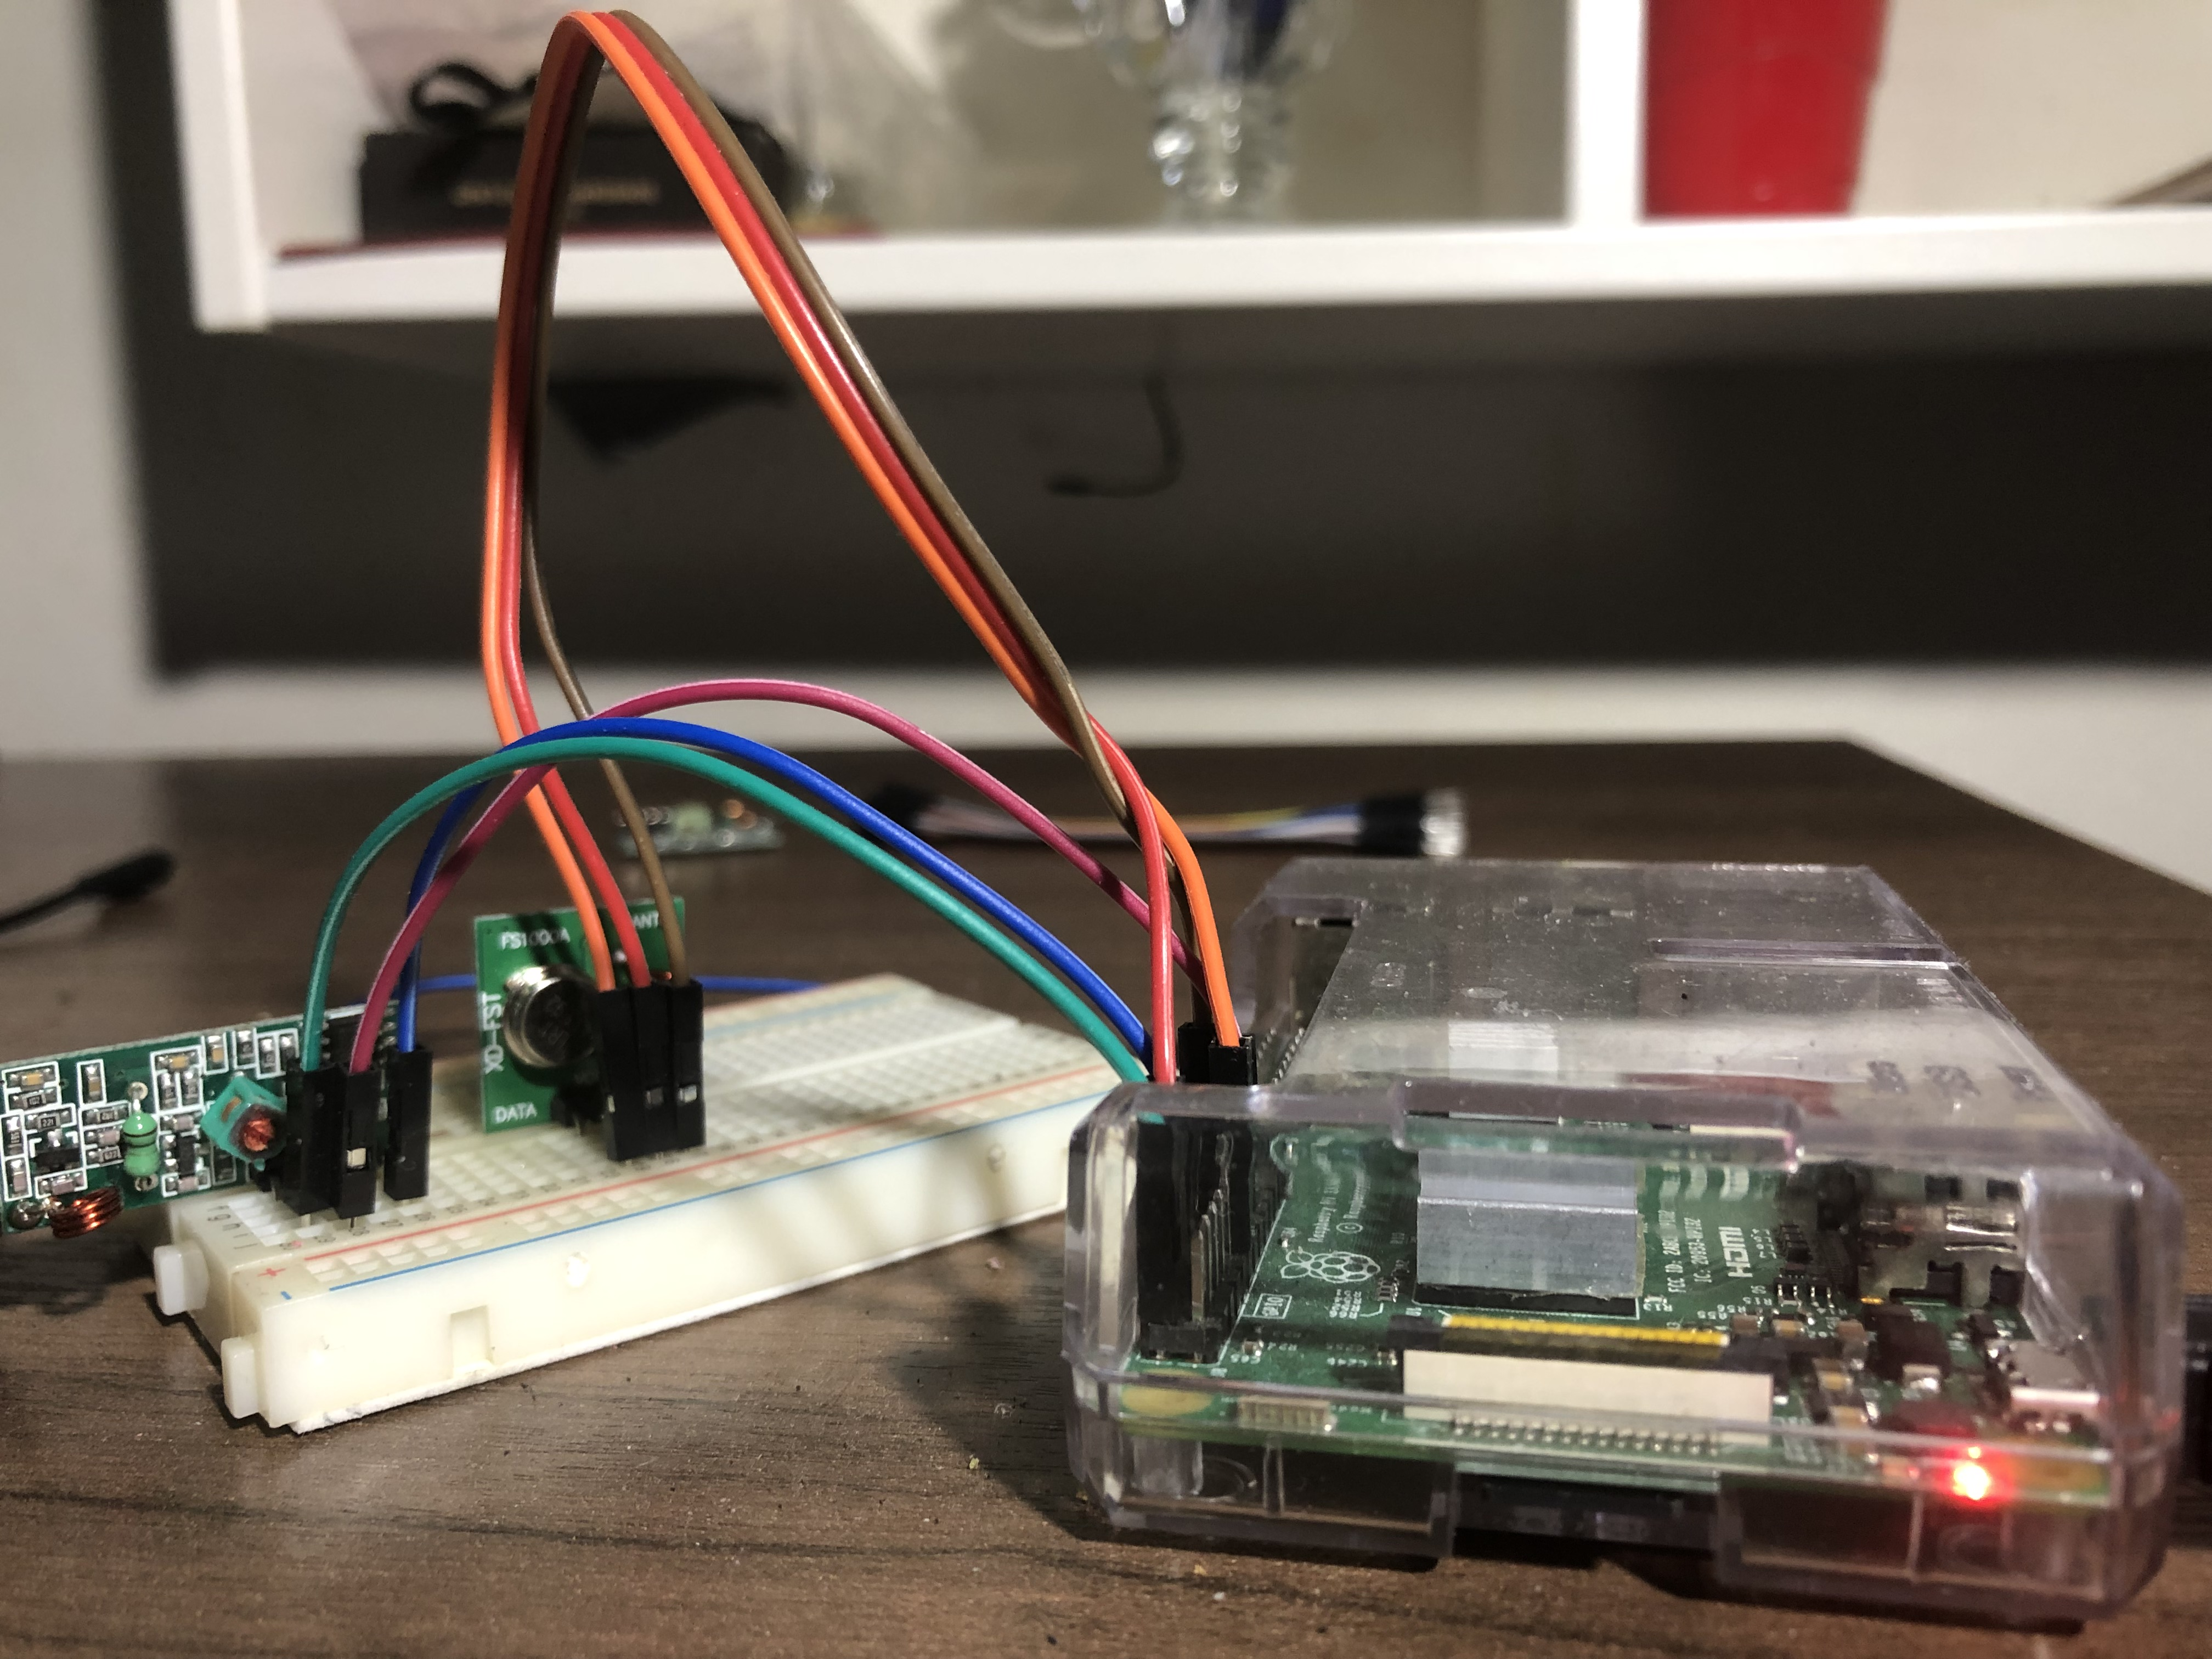
\includegraphics[width=0.5\textwidth]{rf_circuit}
	\caption{Setup for getting RF codes.}
	\label{fig:rf_circuit}
\end{figure}

\end{document}
